\documentclass[12pt]{article}
\usepackage[usenames,dvipsnames]{color}
\usepackage{listings}
\usepackage{graphicx}
\usepackage{fancyhdr}
\usepackage{framed}
\usepackage[T1]{fontenc}
\usepackage[toc,page]{appendix}
\usepackage[utf8]{inputenc}
\usepackage[brazil]{babel}
\usepackage{fancyvrb}
\usepackage[hmargin=2cm,vmargin=2cm]{geometry}
\usepackage{lastpage}
\usepackage{makeidx}
\pagestyle{fancy}

% cabecalho e rodapé
\setlength{\headheight}{120pt}
\setlength{\textheight}{550pt}
\renewcommand{\headrulewidth}{0pt}
\lhead{
\includegraphics[scale=0.03]{brasao.png}}
\rhead{
\includegraphics[scale=0.4]{logo-pnud.png}}
\cfoot{\textbf{\ProjectCode\ - Inovando a democracia participativa}}
\rfoot{\thepage}

\hyphenation{par-ti-ci-pa-ção}
\bibliographystyle{ieeetr}

% definições sobre o autor e o produto
\newcommand{\MyName}{Joenio Marques da Costa}
\newcommand{\MySurnameForename}{Costa, Joenio}
\newcommand{\SupervisorName}{Gabriella Vieira Oliveira Gonçalves}
\newcommand{\MyEmail}{joenio@colivre.coop.br}
\newcommand{\ContractNumber}{2013/000564}
\newcommand{\ContractYear}{2013}
\newcommand{\ProjectCode}{Projeto BRA/12/018}
\newcommand{\NomeSecretaria}{Secretaria Geral da Presidência da República}
\newcommand{\SiglaSecretaria}{SG/PR}
\newcommand{\ProductNumber}{04}
\newcommand{\ProductTitle}{Proposta de aperfeiçoamento para aplicativos de
  participação social}
\newcommand{\ProductSubtitle}{Aperfeiçoamento das trilhas de participação e
  interface de gestão dos aplicativos de participação social}
\newcommand{\ProductDescription}{"Documento com proposta de aperfeiçoamento
  para os aplicativos das trilhas de Participação Social, com propostas de
  funcionalidades e exemplos de códigos."
}
\newcommand{\ProductValue}{R\$ 10.800,00 (dez mil e oitocentos reais)}
\newcommand{\ObjetoContratacao}{"Construção dos códigos para comunidades e
  aplicativos do portal da participação social."
}
\newcommand{\DataEntrega}{?? Setembro de 2014}
\newcommand{\PalavrasChave}{palavra1, palavra2, palavra3, etc}

% lista de abreviações
\makeindex

\begin{document}

\newgeometry{hmargin=3cm,vmargin=1.5cm}
\begin{center}
\thispagestyle{empty}
{\color{MidnightBlue}


\includegraphics[scale=0.9]{logo-pnud.png}

\vspace{4cm}

{\bf \large \ProjectCode\ - Desenvolvimento de Metodologias
de Articulação e Gestão de Políticas Públicas para Promoção da Democracia
Participativa}

\vspace{1.5cm}

{\bf \large Produto \ProductNumber\ -\ \ProductTitle}

\vspace{1.5cm}

\ProductSubtitle

\vspace{4cm}

\MyName

\vspace{2cm}

}


\includegraphics[scale=0.04]{brasao.png} \\
{\bf \small \NomeSecretaria}

\end{center}
\restoregeometry
\newpage

\newgeometry{hmargin=3cm,vmargin=1.5cm}
\addtolength{\topmargin}{2.5cm}
\thispagestyle{empty}
{\color{MidnightBlue}

{\bf \LARGE Produto \ProductNumber\ -\ \ProductTitle}

\hrulefill

\vspace{1cm}

\begin{center}

{\bf \large Contrato n. \ContractNumber}

\vspace{1.5cm}

{\bf \large Objeto da contratação: \ObjetoContratacao}

\end{center}

\vspace{3.2cm}

Valor do produto: \ProductValue

\vspace{1.2cm}

Data de entrega: \DataEntrega

\vspace{1.2cm}

Nome do consultor: \MyName

\vspace{1.2cm}

Nome do supervisor: \SupervisorName

}

\vspace{2cm}

\begin{center}

\includegraphics[scale=0.04]{brasao.png} \\
{\bf \small \NomeSecretaria}
\end{center}

\restoregeometry
\newpage

\newgeometry{hmargin=3cm,vmargin=1.5cm}
\addtolength{\topmargin}{5cm}
\thispagestyle{empty}

\begin{framed}

{\raggedright \MySurnameForename} \\

\ProductTitle: \ProductSubtitle\ / \ContractYear. \\

Total de folhas: \pageref{LastPage} \\

\vspace{1cm}

Supervisor: \SupervisorName \\

\SiglaSecretaria \\

\NomeSecretaria \\

Palavras-chave: \PalavrasChave. \\

\end{framed}

\vspace{3cm}

{\raggedright 
\includegraphics{licenca-cc-by-nc.png} \ Esta obra é licenciada sob
uma licença Creative Commons - Atribuição-NãoComercial. 4.0 Internacional.}

\restoregeometry
\newpage

\tableofcontents
\newpage

\begin{abstract}
escrever resumo aqui... \\

{\bf Palavras-chave:} \PalavrasChave.
\end{abstract}
\newpage

\section{Introdução}

Em consonância com os objetivos e cronograma previsto no âmbito do
projeto BRA/12/018:
\textbf{Desenvolvimento de Metodologias de Articulação e Gestão de
Políticas Públicas para Promoção da Democracia Participativa},
firmado entre a Secretaria-Geral da Presidência da República
(SG/PR) e o Programa das Nações Unidas para o Desenvolvimento (PNUD),
o presente documento apresenta \ProductDescription.

Essa proposta está configurada como produto \ProductNumber~da consultoria técnica
para especificação da construção dos códigos das metodologias de
organização da informação e interação participativa do portal de
participação social.

\section{Desenvolvimento}

O Participa.br é a Plataforma Federal da Participação Social. Trata-se de mais
um espaço para participação social no Brasil, escuta e diálogo entre o Governo
Federal e a Sociedade Civil. 

A plataforma, totalmente desenvolvida em software livre, tem como missão
desenvolver práticas inovadoras de participação via internet e oferta de
espaços de manifestação e debate para qualquer cidadão ou organização, com o
intuito de construir políticas públicas cada vez mais eficazes e efetivas.

O Participa.br é desenvolvido sob a plataforma para redes sociais Noosfero.

\subsection{O Noosfero}

O Noosfero é uma plataforma web livre para redes sociais e de economia
solidária que possui as funcionalidades de Blog, e-Portfolios, CMS, RSS,
discussão temática, agenda de eventos e inteligência econômica colaborativa
num mesmo sistema! O Noosfero utiliza a linguagem de programação Ruby com
framework Rails e, portanto, suporta bancos de dados, PostgreSQL, MySQL,
SQLite entre outros.

Noosfero é um Software Livre e licenciado sob a GNU Affero General Public
License (AGPL), versão 3\cite{wikipediaSingleSignOn}.

\subsection{Aperfeiçoamento para os aplicativos de Participação Social}

\subsubsection{Observatório do Participa.br}

O Participa.br organiza seus debates em torno de comunidades temáticas criadas
a partir do interesse da sociedade ou governo. A gestão das comunidades é
conjunta. A construção de um processo participativo dentro de uma comunidade
ocorre através de criação de diversos tipos de conteúdos e ferramentas
digitais de participação. Estes conteúdos e ferramentas podem ser criados por
qualquer usuário do ambiente participativo e possuem em comum 2 informações de
vital importancia para dar sustentação ao observatório aqui proposto, são
elas: tags e categorias (ver Figura~\ref{categorias-tags}), elas dão um viés
estrutural a todo conteúdo e ferramenta de participação criada no
Participa.br.

\begin{figure}[h]
\center
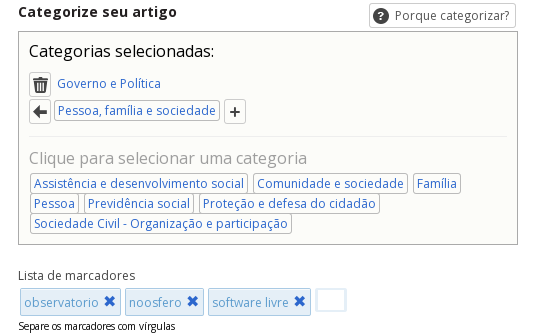
\includegraphics[scale=0.6]{categorias-tags.png}
\caption{Definição de categoria e tag na edição de conteúdo}
\label{categorias-tags}
\end{figure}

O observatório do Participa.br dará aos usuários uma forma de acompanhar temas
de interesse através da seleção de tags (ver Figura~\ref{observatorio-tags}) e
categorias (ver Figura~\ref{observatorio-categorias}), isto proporcionará ao
usuário uma visão personalizada de tudo que acontece no Participa.br (ver
Figura~\ref{observatorio-busca}).

\begin{figure}[h]
\center
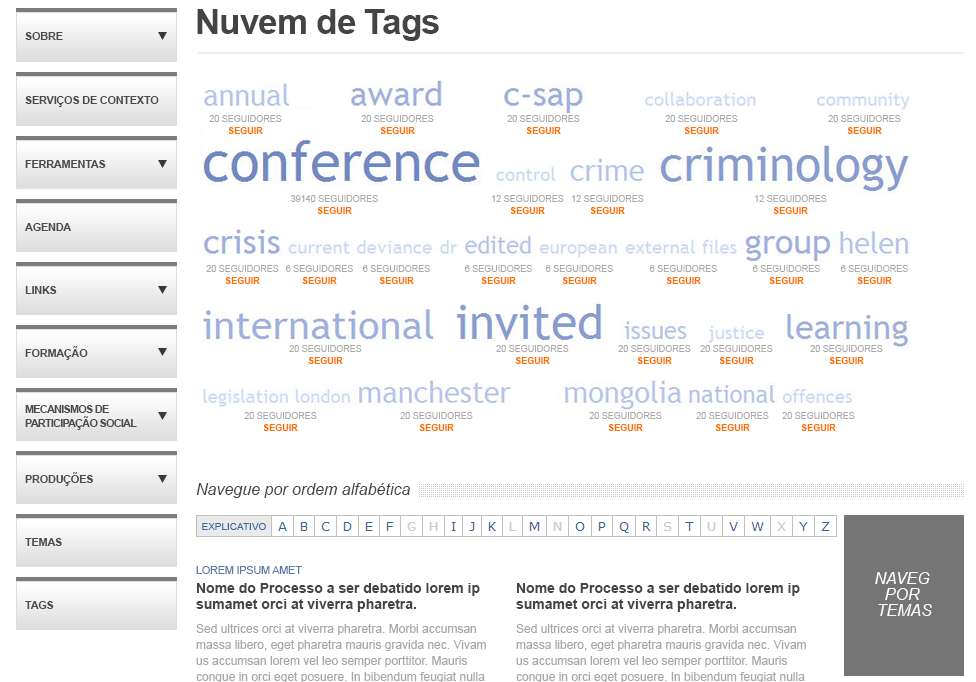
\includegraphics[scale=0.4]{observatorio-tags.png}
\caption{Seleção de tags para acompanhar no observatório}
\label{observatorio-tags}
\end{figure}

\begin{figure}[h]
\center
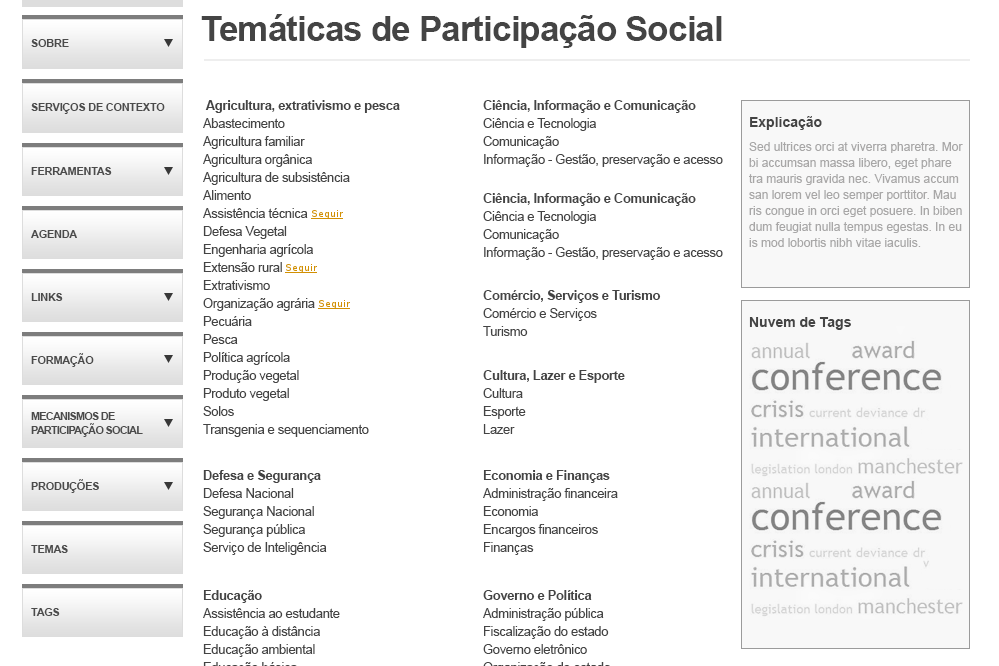
\includegraphics[scale=0.4]{observatorio-categorias.png}
\caption{Seleção de categorias para acompanhar no observatório}
\label{observatorio-categorias}
\end{figure}

\begin{figure}[h]
\center
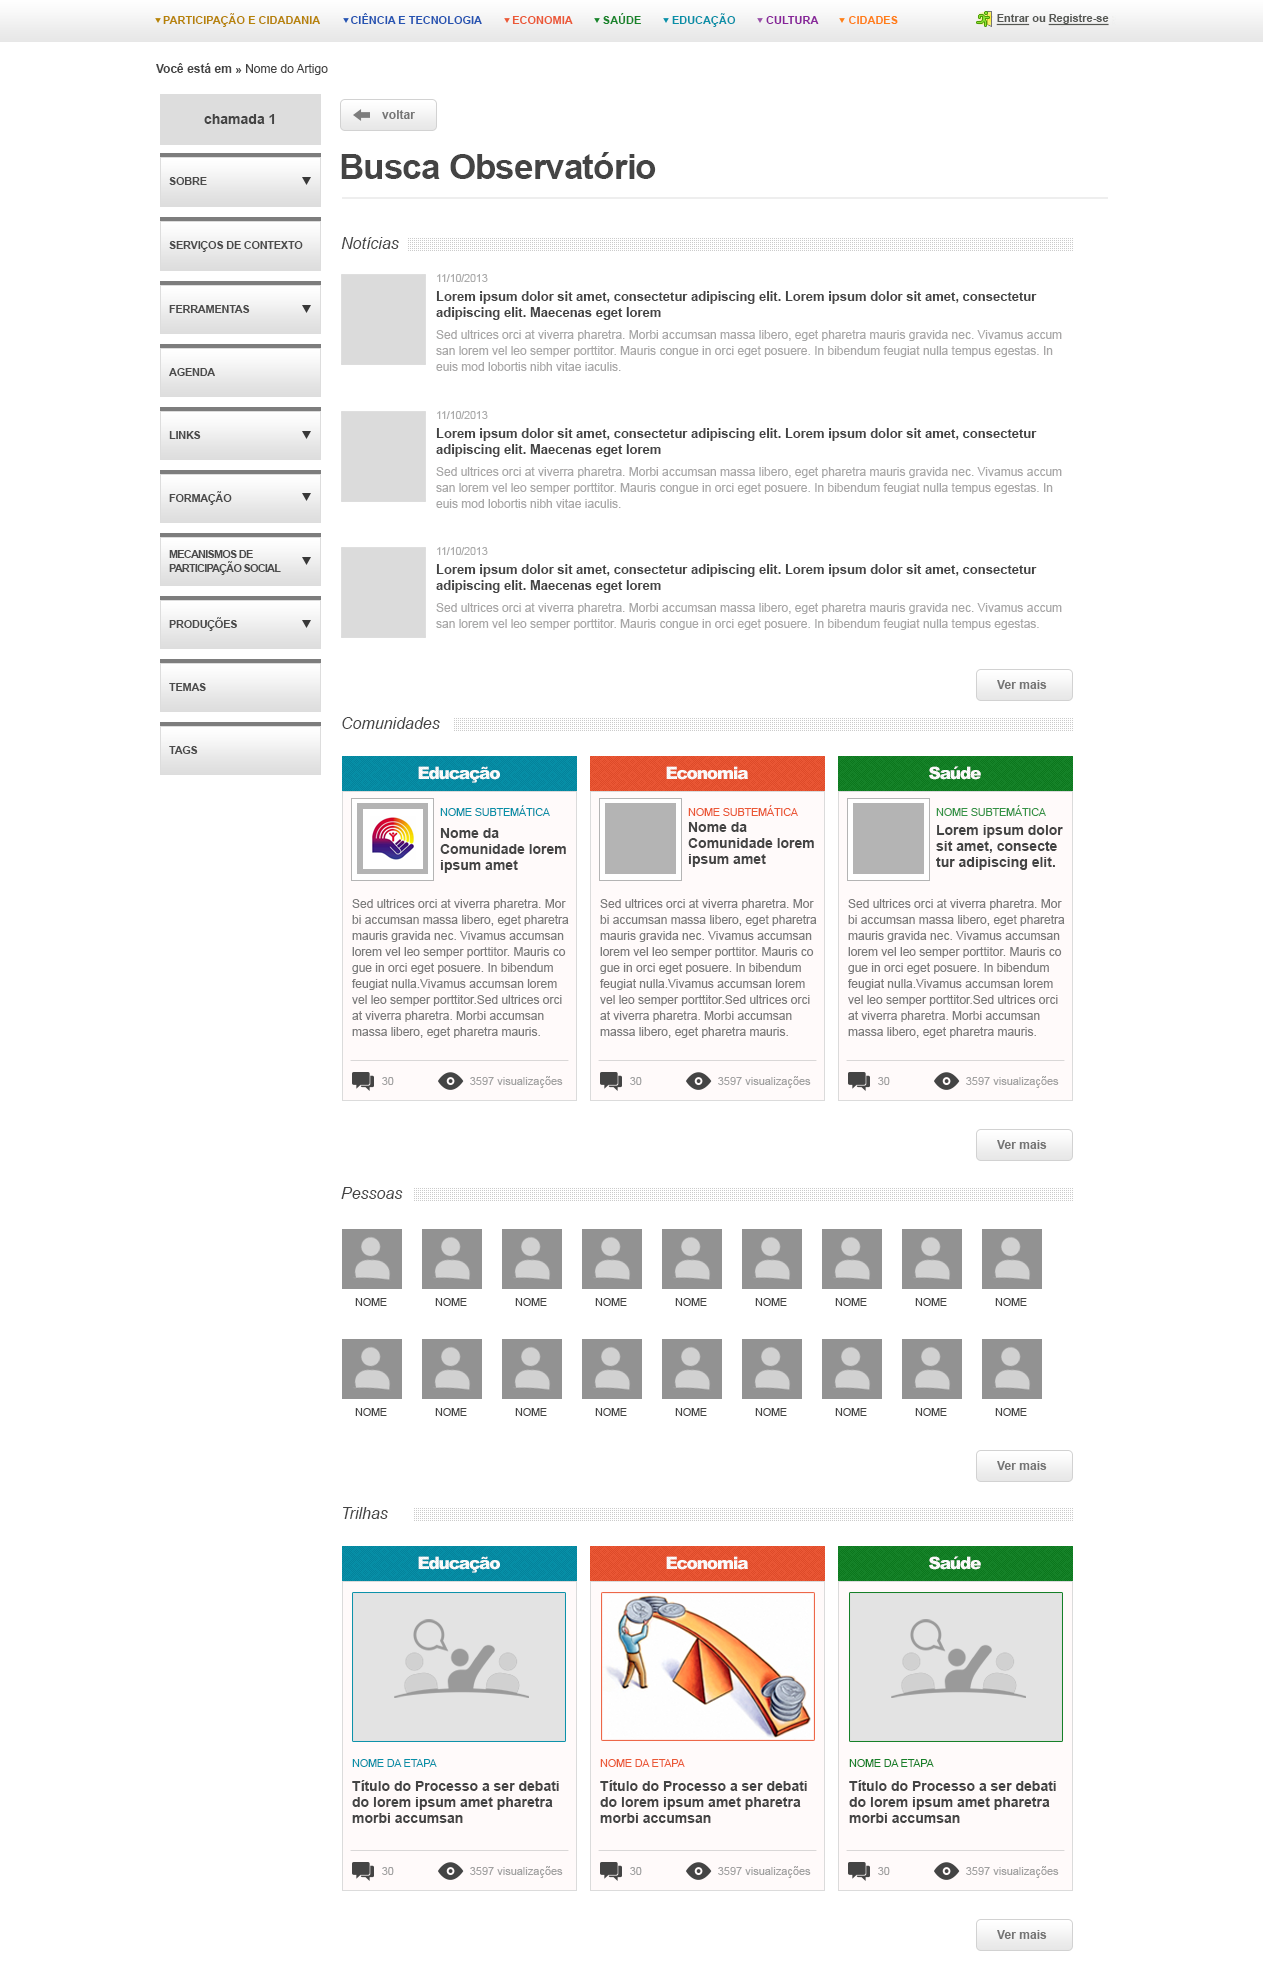
\includegraphics[scale=0.25]{observatorio-busca.png}
\caption{Observatório - Página de busca principal}
\label{observatorio-busca}
\end{figure}

Será possível ainda, acompanhar o observatório a partir de leitor de feeds
externos, pois será disponibilizado um FEED RSS a partir dos conteúdos do
observatório conforme pode ser visto na Figura~\ref{observatorio-wireframe}.

\begin{figure}[h]
\center
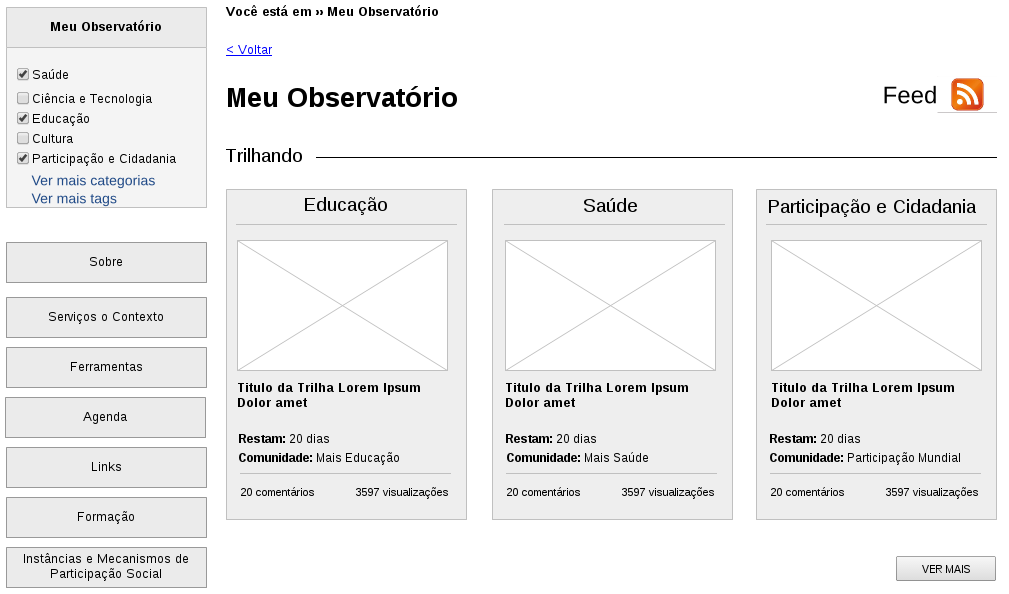
\includegraphics[scale=0.5]{observatorio-wireframe.png}
\caption{Observatório - Página de busca com opções de filtros}
\label{observatorio-wireframe}
\end{figure}

Para possibilitar a implementacao do observatorio sera preciso:
\begin{itemize}
  \item Criar uma forma de visuzlizacao de todas as categorias assim como há para tags
  \item Permitir aos usuarios seguir tags e categorias
  \item Implementar uma nova funcionalidade que permita ao usuário visualizar conteúdos com base nas tags e categorias que está seguindo
\end{itemize}

Issues relacionadas ao observatório:
\begin{itemize}
  \item https://gitlab.com/participa/noosfero/issues/66
\end{itemize}

Mais wireframes sobre esta feature em:

\begin{itemize}
  \item http://sgpr.faracy.com.br/wireframe/Meu\%20Observatorio.html
  \item http://sgpr.faracy.com.br/wireframe/Lista\%20de\%20Temas\%2029-09.html
  \item http://sgpr.faracy.com.br/wireframe/Nuvem\%20de\%20Tags\%2027-09.html
\end{itemize}

\subsubsection{Painel gestor das ferramentas de consulta}

Painel administrativo e de sistematização para as ferramentas de comentários
por trecho e por parágrafo através de etiquetas e status para sistematização e
outras funcionalidades.

Para possibilitar tal sistematização é preciso habilitar o plugin
CommentClassification\cite{commentClassificationPlugin} no Noosfero, plugin
que possibilita classificar plugins através de etiquetas e tags. Os usuários
podem indicar semanticamente qual o significado do seu comentário no momento
em que o faz, como pode ser visto na Figura~\ref{etiqueta}.

\begin{figure}[h]
\center
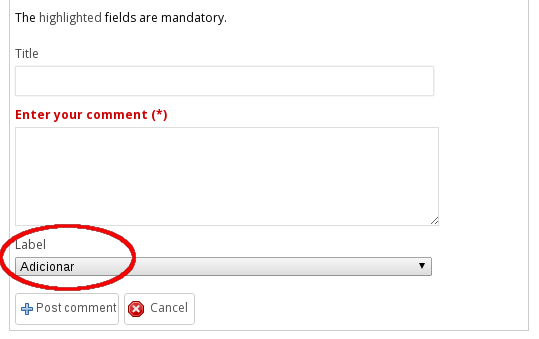
\includegraphics[scale=0.5]{etiqueta.png}
\caption{Etiquetas de classificação para comentários}
\label{etiqueta}
\end{figure}

Clicando em configuração, o administrador poderá gerenciar as "labels" (as
etiquetas) e os "Status" (que o avaliador vai escolher e dar a justificativa)
(ver Figuras \ref{manage-labels} e \ref{manage-status}).

\begin{figure}[h]
\center
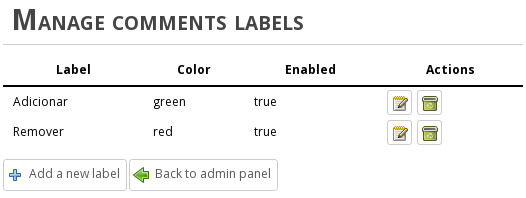
\includegraphics[scale=0.5]{manage-labels.png}
\caption{Gerenciamento de labels do plugin CommentClassification}
\label{manage-labels}
\end{figure}

\begin{figure}[h]
\center
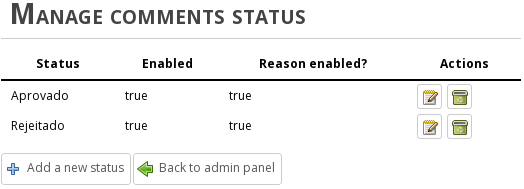
\includegraphics[scale=0.5]{manage-status.png}
\caption{Gerenciamento de status do plugin CommentClassification}
\label{manage-status}
\end{figure}

Desta forma o administrador da consulta pode pré-definir etiquetas que serão
utilizadas pelos usuário no momento do comentário, o administrador pode por
exemplo criar etiquetas que indiquem:

\begin{itemize}
  \item Adição ou remoção de texto
  \item Concordancia ou discordancia
  \item Opinião sobre qualidade do texto (bom, ruim, etc)
  \item Dentre outros, a criação de etiquetas é livre e o admin pode criar quantas quiser
\end{itemize}

O administrador da consulta pode a partir do painel de controle de uma
comunidade como na Figura~\ref{control-panel} gerenciar os comentários e
definir status para eles, estes status são pré-definidos através da
configuração do plugin.

\begin{figure}[h]
\center
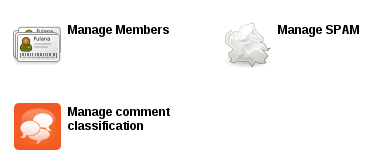
\includegraphics[scale=0.5]{control-panel.png}
\caption{Imagem no painel de controle da comunidade}
\label{control-panel}
\end{figure}

Deve existir no painel a opção de exportação em CSV dos trechos, comentários,
status, justificativas e novas redações.

Como um trecho pode ter vários comentários e cada comentário pode ter várias
sugestões de justificativas e alteração de texto, vê se dessa forma está bem
organizado. (colocar imagem de comentários aninhados)

\begin{figure}[h]
\center
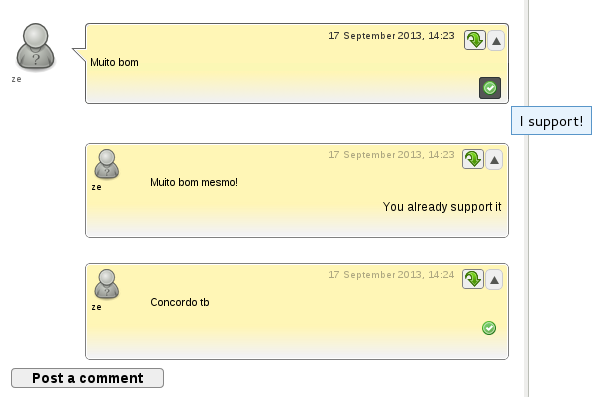
\includegraphics[scale=0.5]{support-on-comment.png}
\caption{Apoio/aprovo este comentario}
\label{support-on-comment}
\end{figure}

Agora o foco mesmo é o painel de sistematização das consultas, aquele que vc já está trabalhando.

http://noosfero.org/Development/ActionItem2520

Este recurso de marcar etiquetas e status em comentários pode ser utilizado em
conteúdos padrão do Noosfero e também em artigos com comentários por parágrafo
ou trecho, para estes 2 últimos pode se fazer necessário a união de duas
unidades comentáveis e para isto basta englobar os trechos e referenciar o
código do trecho precedido de virgula; Exemplo: \[commentable name="p1,p2"\] o
que significa: p1 paragrafo 1 e p2 paragrafo 2... Assim todos os comentários
são listados de forma unificada para os dois parágrafos e somente será exibido
uma unidade comentável.

%O plugin permite que especifique o texto original através da tag
%\[original\_version\], isso se faz importante quando o usuário tem que fazer alguma comparação entre o que esta sendo consultado com a versão anterior da consulta.

É obrigatório para o plugin marcar identificadores na tag comentável; é
através destes identificadores que filtramos informações e acompanhamos uma
consulta; a criação desses identificadores tem sido de livre uso para o
administrador e geralmente esta associada e ou referenciada ao trecho
comentável, exemplo: p1 = paragrafo 1.. art2 = artigo 2... cap1 = capitulo 1.

- Para criar/editar/remover uma label:
http://sgpr.colivre.net/admin/plugin/comment\_classification/labels
  * Cada label pode ter uma cor. Essa cor será usada na visualização do comentário. Coloquei as vermelho, verde, amarelo, azul e cinza. Mas podemos colocar mais

- Para criar/editar/remover um status:
http://sgpr.colivre.net/admin/plugin/comment\_classification/status

Tanto os status quanto os labels podem ser "desabilitados", para que as pessoas não possam escolher.

- Ícone no painel de controle para gerenciar a classificação por perfil
http://sgpr.colivre.net/myprofile/compromisso-nacional

Criei um artigo igual ao da consulta:
http://sgpr.colivre.net/compromisso-nacional

Em cada comentário tem o link "I support!" que seria o "Curtir" do facebook.
E também tem o "Add status", que só é visto pelas pessoas com permissão de "moderar comentários"

* O que falta:
 -  Fazer a tela para mostrar as estatísticas na própria ferramenta: qtos querem adicionar, suprimir, questionamentos etc
 -  A opção de sugestão que pode ser incorporada ao texto dá para classificar como viável e colocar na justificativa a alteração do texto. Mas falta definir um atributo ou algo assim pra que essa informação apareça diferente no histórico de avaliações
 - O botão para um avaliador poder concordar com a justificativa de outro avaliador
 - Mostrar o trecho que está sendo comentado.
 - Ícone do "I support"
 - Melhor organização das 3 novas informaçõs nos comentários (label, status, support)
 - Ícone no painel de controle para visualizar a classificação dos comentários
 - Permitir que uma comunidade desative a função no perfil dela, mesmo estando ativo no ambiente
 - Gerar um .odt com as informações

===========================================================

Sim, aqui fabiano tb pode propor. É importante que a interface indique de forma clara os comentários que já passaram por "colocação de status" incentivando a equipe de sistematização a responder todos. Podia ser uma "mascara" de cor em cima do avatar do comentador, ou outra solução que possa ser bem visível. 

Para exibição dos status, justificativas e novas redações acredito que a melhor solução seja mesmo aquelade duas colunas: 1) Coluna da direita a minuta com os blocos e trédis de comentários 2) Coluna daesquerda as "trédis de status/históricos" do comentário em "foco".
 
 - Ícone no painel de controle para visualizar a classificação dos comentários
 - Permitir que uma comunidade desative a função no perfil dela, mesmo estando ativo no ambiente
 - Gerar um .odt com as informações

Acho importante incluir no painel a opção de exportação em CSV dos trechos, comentários, status, justificativas e novas redações.
 
https://gitlab.com/participa/noosfero/issues/33

================================

O Participa.br conta com inúmeras ferramentas de consulta pública e
participação popular, como:

* Ferramenta para construçao e debates de propostas (referencia produto3 joenio)
* Ferramenta de comentários por parágrafos (Comment Group Plugin)
* Comentários em artigos e comentário por trecho
* Votação de artigos/conteúdos (Vote Plugin)

%=============================================
%Criar issue para "citar" pessoas nos comentários, conteúdo também, exemplo facebook.
%Mostrar um link e balãozinho nestas citações, criar um alerta para a pessoa que foi citada.
%===============================================================

\section{Conclusão}

Neste documento foi apresentado um \ProductDescription

Lembramos que para tornar o Portal de Consulta Pública realmente um canal de
consulta e participação popular na discussão e na definição da agenda
prioritária do país, é necessário que além de documentação faça-se um esforço
de movimentar as pessoar fora do ambiente virtual, para que haja um
engajamento no uso e contribuição deste projeto de forma consistente e perene.

\newpage
\bibliography{bibliografia}
\newpage
\listoffigures
\newpage
\printindex
\newpage
\definecolor{lightgrey}{rgb}{0.95,0.95,0.95}
\lstset{language=Ruby,basicstyle=\small\ttfamily,backgroundcolor=\color{lightgrey}}

\section{Anexos}

\subsection{Exemplo de código do plugin Noosfero para pairwise}

\lstinputlisting{pairwise_content.rb}

\subsection{Exemplo de código XML retornado pelo pairwise-api}

\begin{lstlisting}
<?xml version="1.0" encoding="UTF-8"?>
<prompt>
  <created-at type="datetime">2010-07-01T23:48:01+00:00</created-at>
  <id type="integer">1</id>
  <left-choice-id type="integer">10</left-choice-id>
  <question-id type="integer">7</question-id>
  <right-choice-id type="integer">9</right-choice-id>
  <tracking nil="true"></tracking>
  <updated-at type="datetime">2010-07-01T23:48:01+00:00</updated-at>
  <votes-count type="integer">0</votes-count>
  <left-choice-text>bar</left-choice-text>
  <right-choice-text>foo</right-choice-text>
</prompt>
\end{lstlisting}

%\appendix
%\appendixpage
%\section{Foo bar}
\label{foobar}

%\lstinputlisting{observatorio.rb}


\end{document}
